\documentclass[10pt]{scrreprt}
\usepackage[a4paper, top=30mm, left=25mm, right=25mm, bottom=30mm]{geometry}
\usepackage[utf8]{inputenc}

\usepackage[Bjornstrup]{fncychap}
\usepackage{ngerman}
\usepackage{graphicx}
\usepackage{epstopdf}
\usepackage{etoolbox}
\usepackage{enumitem}
\usepackage{url}
\usepackage{numprint}
\usepackage{longtable}
\usepackage{tabu}
\usepackage{multirow}
\usepackage{caption}
\usepackage{array}
\usepackage{amssymb}


\makeatletter
\patchcmd{\@makechapterhead}{\vspace*{50\p@}}{\vspace*{-20\p@}}{}{}
\patchcmd{\@makeschapterhead}{\vspace*{50\p@}}{\vspace*{7\p@}}{}{}
\patchcmd{\DOTIS}{\vskip 40\p@}{\vskip -12\p@} 
\makeatother
  
\captionsetup[figure]{labelfont={sf,bf},textfont={sf}}
\deffootnotemark{[\thefootnotemark]}
\deffootnote{1.5em}{1em}{[\thefootnotemark] }
\setlength{\parindent}{0pt}
\renewcommand{\labelitemi}{ \raisebox{0.3ex}{\small$\blacktriangleright$} }

\newcommand{\sfbf}[1]{\textbf{\sffamily #1}}
\newcommand{\sfit}[1]{\textit{\sffamily #1}}
\newcommand{\W}{\sfbf{W}}
\newcommand{\ziel}[1]{{\fontsize{9.5}{11}\textsf{/#1/}}}
\newcommand{\ziellabel}{Z}
\newcommand{\muss}{\renewcommand{\labelenumi}{\textbf{\ziel{\ziellabel\numprint{\theenumi}0}}}}
\newcommand{\wunsch}{\renewcommand{\labelenumi}{\textbf{\ziel{\ziellabel\numprint{\theenumi}0W}}}}
\newcommand{\JoglEarth}{\raisebox{-1.2mm}{
\includegraphics[scale=0.33]{Logo-Text.eps}} }
\newcommand{\textref}[1]{\mbox{\raisebox{0.1ex}{\small$\rightarrow$ }\textit{#1}}}

\newenvironment{details}[1][6pt]{%
  \parskip#1 \parindent6mm \raggedright%
  \def\item{\par\ignorespaces\hangindent=5mm \hangafter1}}{%
  \par\ignorespaces} 
  

\begin{document}

\thispagestyle{empty}
\sffamily
 
\title{Pflichtenheft}

\begin{figure}
\begin{flushright}
	
\includegraphics[scale=0.4]{uniLogo.eps}
\vspace{2.0 cm}
\end{flushright}
\end{figure}

\begin{center}
\vspace{2.0 cm}
{\LARGE SEP – Wintersemester 2013/14}

\vspace{1.0 cm}
\textbf{{\Huge Pflichtenheft}}

\vspace{0.8 cm}
\begin{figure}[!htb]
\begin{center}
	%
\includegraphics[scale=1.0]{projektLogo.eps}
	
\includegraphics[scale=1.5]{Logo-Print.eps}
\end{center}
\end{figure}

\vspace{0.2 cm}
\textbf{{\huge OpenStreetMap: Die Welt in 3D}}

\vspace{1.5 cm}
31.10.2013

\vspace{0.5 cm}
Version: 1.1

\vspace{1.5 cm}
{\Large Projektbetreuer: Peter Barth}

\vspace{1.5 cm}
\begin{tabular}{|c|c|c|}
\hline 
\rule[-1ex]{0pt}{4ex} \textbf{Phase} & \textbf{Verantwortlicher} & \textbf{E-Mail Adresse} \\ 
\hline  \hline
\rule[-1ex]{0pt}{4ex} Pflichtenheft & Gabriele Haas & haasgab@fim.uni-passau.de \\ 
\hline  \hline
\rule[-1ex]{0pt}{4ex} Entwurf & Thomas Eder & ederthom@fim.uni-passau.de \\ 
\hline  \hline
\rule[-1ex]{0pt}{4ex} Spezifikation & Christof Blauberger & blauberg@fim.uni-passau.de \\ 
\hline  \hline
\rule[-1ex]{0pt}{4ex} Implementierung & Fabian Knorr & knorrfab@fim.uni-passau.de \\ 
\hline \hline 
\rule[-1ex]{0pt}{4ex} Testing & Constantin Wenger & wengerco@fim.uni-passau.de \\ 
\hline  \hline
\rule[-1ex]{0pt}{4ex} Präsentation & Sebastian Reichl & reichlse@fim.uni-passau.de \\ 
\hline 
\end{tabular}

\end{center}


\pagebreak
\rmfamily
\tableofcontents


\chapter{Ausgangssituation}
Die Karten des OpenStreetMap-Projekts erfreuen sich immer größerer Beliebtheit. Der Detailgrad, die Menge an verschiedenen Merkmalen und die Genauigkeit der Daten sind die ihrer Konkurrenz in den meisten Regionen der Welt weit voraus. Durch die große Auswahl an Informationen und die Flexibilität in der Darstellung eröffnen sich unzählige Anwendungsmöglichkeiten.

Die Grafikleistung einfacher Desktoprechner ist bereits für aufwändige 3D-Szenarien ausgelegt. Die Ansprüche der Benutzer hat sich in den letzten Jahren dahingehend geändert, dass ansprechende visuelle Gestaltung und einfache Bedienung ausschlaggebend für die Wahl eines Softwareproduktes ist.

\vspace{0.5cm}

Die Projektion einer Straßenkarte auf einen dreidimensionalen Globus ist die intuitivste und geographisch korrekteste Darstellung. Es liegt also nahe, auf dieser Grundlage eine Anwendung zur Kartenanzeige zu entwickeln.

Da bereits Projekte mit einem gleichen oder ähnlichen Ziel existieren, möchten wir uns von diesen durch die folgenden Schwerpunkte abgrenzen:
\begin{itemize}
\item Verwendung der freien Kartendaten des OpenStreetMap-Projekts
\item Realisierung einer dreidimensionalen Globusoberfläche mit den Höhendaten der NASA
\item Intuitive Bedienung der Anwendung ohne Einarbeitungszeit
\item Die Möglichkeit der spielerischen Benutzung durch Kinder ohne nennenswerte PC-Kenntnisse
\item Vollständige Plattformunabhängigkeit durch Java
\item Effiziente Speicher- und Bandbreitennutzung
\end{itemize}

\vspace{0.5cm}

Basierend auf diesen Grundprinzipien wird in diesem Pflichenheft das Konzept der Desktopanwendung \JoglEarth entwickelt.




\chapter{Produkteinsatz}
\section{Anwendungsbereich}
\JoglEarth soll eine dreidimensionale Ansicht der Welt sowie eine ebene Kartenansicht bieten. Beides erfolgt auf Basis des OpenStreetMap-Projekts und Satellitendaten der NASA. \\

Die grafische Benutzeroberfläche zeigt dafür im dreidimensionalen Modus eine Weltkugel, die frei gedreht und gezoomt werden kann, und im zweidimensionalen einen Ausschnitt der Weltkarte. Die Karte kann aus verschiedenen Kategorien wie Satellitenbildern oder Straßenkarten gewählt werden. Die Steuerung erfolgt mit Tastatur und Maus. \\

Mit einer Suchfunktion kann im Umkreis oder global nach Orten gesucht werden. Punkte besonderen Interesses wie Tankstellen oder Banken können über dem Kartenbild eingeblendet werden.

\section{Zielgruppe}
Primäre Zielgruppe des Systems sind Privatanwender, die eine andere Art der Kartendarstellung als die typischen Onlinekarten bevorzugen. \\

Auch soll die Anwendung wissbegierige Kinder ansprechen. Voraussetzung ist lediglich der geübte Umgang mit der Maus und/ oder Tastatur.


\section{Sicherheit, Datenschutz}
Die Anwendung wahrt von vorne herein die Sicherheit des Systems und schützt die Privatsphäre des Nutzers. Da sie keine sicherheitskritischen Daten verarbeiten muss, ist dies implizit gegeben und stellt keine besondere Anforderung an den Entwurf dar.
\begin{itemize}
\item Es ist weder zur Bedienung, noch zum Beschaffen der Kartendaten eine Authentifikation erforderlich 
\item Es werden keine persönlichen Daten des Anwenders über das Netz übertragen
\item Es wird kein Code aus dem Netz nachgeladen und ausgeführt
\item Das Programm hat keine (unter Umständen angreifbare) Serverfunktionalität
\end{itemize}

\pagebreak
\section{Lizenzen}
Wird das Produkt veröffentlicht, so müssen die Lizenzen der verwendeten Bibliotheken und Datenquellen berücksichtigt werden:
\begin{itemize}
\item Die Teile der JOGL-Bibliothek sind unter mehreren Versionen der BSD-Lizenz, der SGI Free Software License und der Apache-Lizenz, der Ubuntu Font License und mehreren proprietären Lizenzen veröffentlicht. Details dazu finden sich bei  \footnote{\url{https://jogamp.org/git/?p=jogl.git;a=blob;f=LICENSE.txt}}.
\item OpenStreetMap ist „OpenData“ im Sinne der Open Database Lizenz (ODbL). Die Kartenkacheln stehen unter der Linzenz  Creative Commons „Namensnennung, Weitergabe unter gleichen Bedingungen" 2.0 (CC BY-SA). Weitere Infos, wie auch eine Vorgabe zum Hinweisen auf der Urheberschaft des OSM-Projekts finden sich bei \footnote{\url{http://www.openstretmap.org/copyright}}.
\item Die Daten der Overpass API sowie Nominatim stehen ebenfalls unter der ODbL.
\item Die Satellitenbilder der NASA sind für die Zwecke des Projekts frei verfügbar und stehen unter der Lizenz, die sich bei \footnote{\url{http://www.nasa.gov/audience/formedia/features/MP_Photo_Guidelines.html}} findet.
\item Die Verwendete GUI-Bibliothek JGoodies Forms steht unter der BSD-Lizenz bei \footnote{\url{http://opensource.org/licenses/bsd-license.html}}.
\end{itemize}




\chapter{Produktumgebung}
\section{Software}
Da das Projekt auf Java setzt, ist es betriebssystemunabhängig. Es muss lediglich das Java Runtime Environment (JRE) in Version 7 sowie ein Fenstersystem und Netzwerkunterstützung zur Verfügung stehen. Zusätzliche Programmbibliotheken, die zum Ausführen des Softwarepakets nötig sind, werden mitgeliefert.\\

Da die Software von Seiten der Entwickler nur auf einem kleinen Teil der möglichen Umgebungen getestet werden kann, sollen mindestens folgende Konfigurationen unterstützt werden:
\begin{itemize}
\item Windows 7 und 8 auf x86{\_}64 mit den Herstellertreibern von nVidia und AMD
\item Linux auf x86{\_}64 mit X.org und proprietären Treibern von nVidia / AMD sowie den freien radeon-Treibern für AMD
\end{itemize}


\section{Hardware}
Wie schon bei der Software der Fall sollte die Anwendung auch mit nahezu allen modernen Desktopsystemen kompatibel sein. Folgende (oder eine gleichwertige) Konfiguration wird jedoch für ein optimales Benutzererlebnis mindestens empfohlen:
\begin{itemize}
\item Dual-Core-Prozessor mit 1 GHz Taktfrequenz
\item 2 Gigabyte RAM
\item 200 Megabyte freier Speicherplatz
\item Grafikkarte: Onboard-Grafik mit OpenGL 2.0-Unterstützung
\item Bildschirm mit 1024x768 Pixeln Auflösung und 24 Bit Farbtiefe
\item Standard-Tastatur und Maus
\end{itemize}



\section{Orgware}
Zum Laden der Kartendaten wird eine durchgehende Internetverbindung benötigt. Um die Wartezeiten akzeptabel zu halten wird mindestens 1MBit/s empfohlen.




\chapter{Zielbestimmungen}

\section{Musskriterien}
\begin{itemize}
\item Intuitiv bedienbare, grafisch ansprechende GUI mit einklappbarer Seitenleiste und Sprachunterstützung für Englisch und Deutsch (siehe \ziel{F010}, \ziel{F020}, \ziel{F030}, \ziel{F040})
\item Bedienung mit Maus und Tastatur (siehe \ziel{F160})
\item Anzeige der momentanen und möglichen Zoomstufen (siehe \ziel{F050})
\item Sinnvolle Beschränkung von Zoom und Beweglichkeit (siehe \ziel{F210})
\item Ladebalken für im Hintergrund geladene Kartendaten (siehe \ziel{F060})
\item Verwendung einer Platzhaltertextur für nicht verfügbare Kacheln (siehe \ziel{F310W})
\item Felder zur Anzeige und Änderung des Längen- und Breitengrads (siehe \ziel{F070})
\item Wechselmöglichkeit zwischen Globus- und flacher Kartenansicht (siehe \ziel{F090})
\item Wechselmöglichkeit zwischen Satellitenbildern und OpenStreetMap-Karten (siehe \ziel{F110})
\item Drehen, Kippen, Zoomen der Ansichten (siehe \ziel{F170}, \ziel{F180})
\item Text- und Symboloverlays für Städte und POIs, Anzeige der Details dazu im Detailfenster (ohne Markierung und Speicherfunktion) (siehe \ziel{F200}, \ziel{F220}, \ziel{F350}, \ziel{F380})
\item Beschränkung der Anzahl gleichzeitig geladener Overpass-Einträge zur Ressourcenschonung (siehe \ziel{F240})
\item Effizientes Laden der Kartendaten durch Caching (siehe \ziel{F250}, \ziel{F260}, \ziel{F270}, \ziel{F280}, \ziel{F290}, \ziel{F300}, \ziel{F330W})
\item Sternenhimmel als Hintergrund (siehe \ziel{F140W})
\end{itemize}

\section{Wunschkriterien}
\begin{itemize}
\item Kinder-Weltkarte als zusätzliche Kartenoption (siehe \ziel{F100W})
\item Sonnensystem-Modellansicht als weiteren Ansichtsmodus (siehe \ziel{F100W}, \ziel{F130W})
\item Anzeige des momentanen Kartenmaßstabs (siehe \ziel{F080})
\item Speicherung der Ansichtseinstellungen (siehe \ziel{F400W})
\item Dreidimensionales Höhenprofil auf Globus- und Kartenoberfläche (siehe \ziel{F120W})
\item Funktion zum Markieren und Speichern von Punkten (siehe \ziel{F190W}, \ziel{F230W}, \ziel{F360W}, \ziel{F390W}, \ziel{F400W})
\item Lokale und Globale Suchfunktion (siehe \ziel{F370W})
\item Aussetzen des Renderns bis zur Bildänderung (siehe \ziel{F340W})
\item Zusätzliche Grafikeinstellungen wie Antialiasing oder Texturfilterung (siehe \ziel{F150W})
\item Vorausladen von Kartendaten an den Rändern der Anzeige und die der nächsten Zoomstufen (siehe \ziel{F320W})
\end{itemize}

\section{Abgrenzungskriterien}
\begin{itemize}
\item Keine Druck- oder Speicherfunktion für Kartenmaterial
\item Keine Exportfunktion für markierte Punkte (Speicherfunktion in externe Datei)
\item Keine dynamischen Flüsse oder andere Animationen
\item Keine Routenplanung
\item Keine Unterstützung für andere als die angegebenen Eingabegeräte
\item Keine Authentifizierung um Zugriff auf vom Benutzer gespeicherte Markierungen zu erhalten
\end{itemize}


\chapter{Benutzeroberfläche}

\section{Visuelles Konzept}

\begin{itemize}
	\item Das Hauptelement der Benutzeroberfläche ist die Karten- oder Globusansicht, die sich im rechten Fensterteil befindet. Der sichtbare Kartenausschnitt kann interaktiv mit Maus oder Tastatur verschoben werden.
	\item Im 2D-Modus zeigt die Ansicht eine Projektion der Karte auf die Ebene, die in der Ansicht nach links/rechts und oben/unten verschoben sowie (perspektivisch) gekippt werden kann.
	\item Im 3D-Modus wird ein Globus gezeigt, auf den das Kartenmaterial projiziert wird. Die Ansicht kann um die Erdachse sowie in Richtung der Pole gedreht; ab einem gewissen Zoomlevel am Kameraursprung gekippt werden.
	\item Am linken Rand des Fensters befindet sich eine Seitenleiste, die sämtliche Steuerungsfunktionen bereitstellt. Der obere Teil ist in Tabs unterteilt, mit denen Funktionen gruppiert werden; der untere Teil zeigt Details zum momentan zentrierten Punkt an.
\end{itemize}


\vspace{1cm}
\begin{figure}[h]
	\centering
	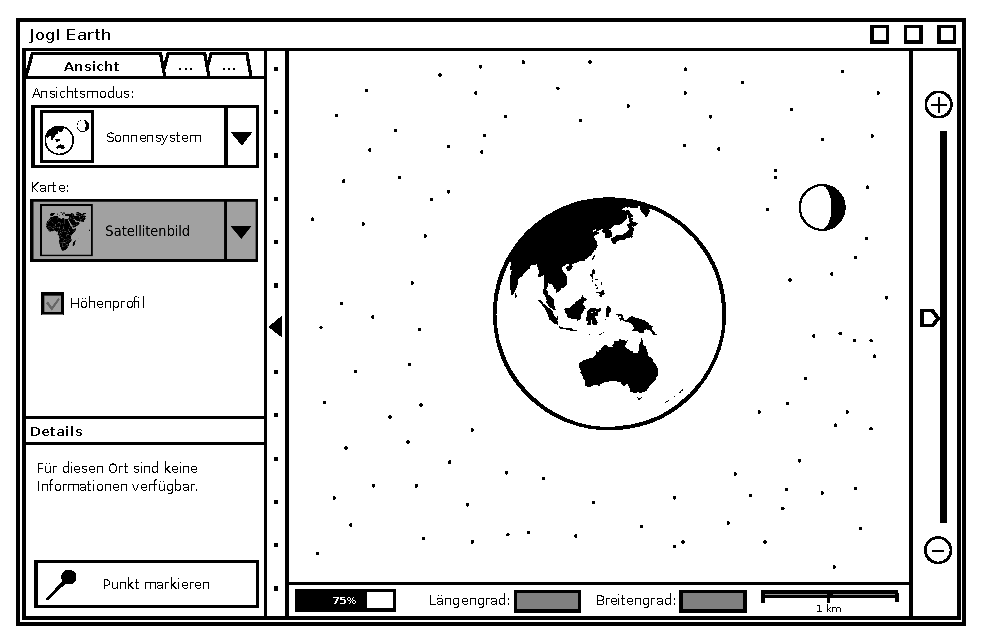
\includegraphics[scale=0.9]{GUI-Sonnensystem.eps}
	\caption{Die Benutzeroberfläche mit geöffnetem Ansichts-Tab im Sonnensystemmodus}
\end{figure}

\begin{figure}
	\centering
	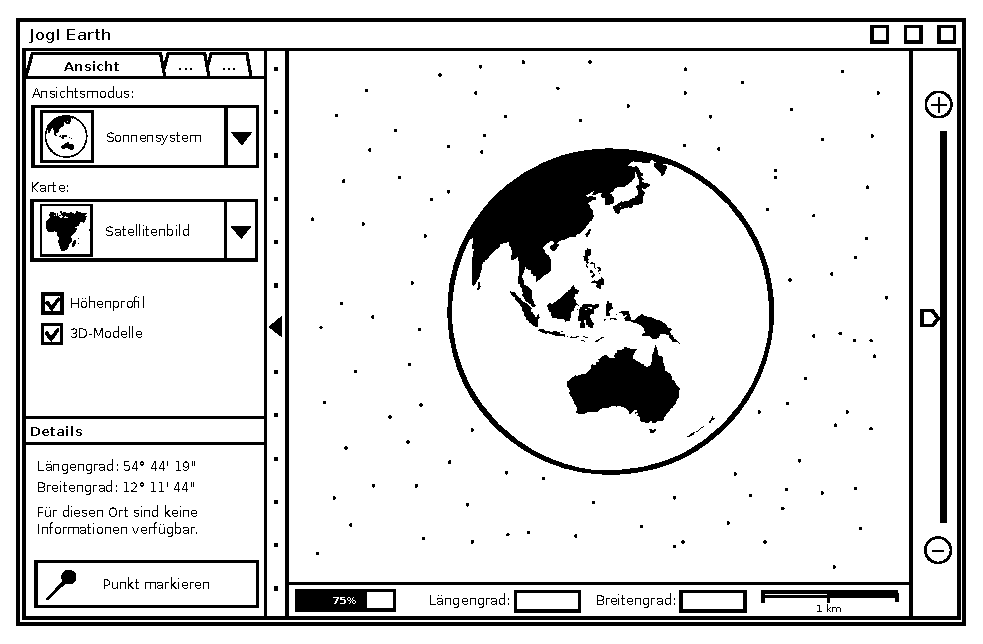
\includegraphics[scale=0.9]{GUI-Ansicht.eps}
	\caption{Die Benutzeroberfläche mit geöffnetem Ansichts-Tab und dargestelltem Globus}
\end{figure}

\begin{figure}
	\centering
	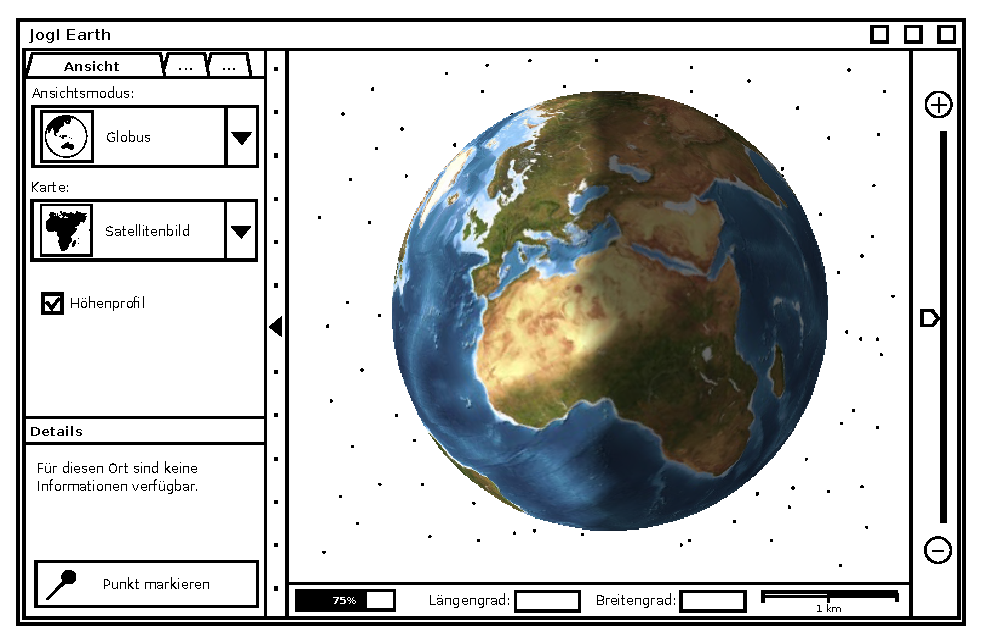
\includegraphics[scale=0.9]{GUI-Ansicht-Welt.eps}
	\caption{Die Benutzeroberfläche mit gewählter Satellitenansicht}
\end{figure}
\begin{figure}
	\centering
	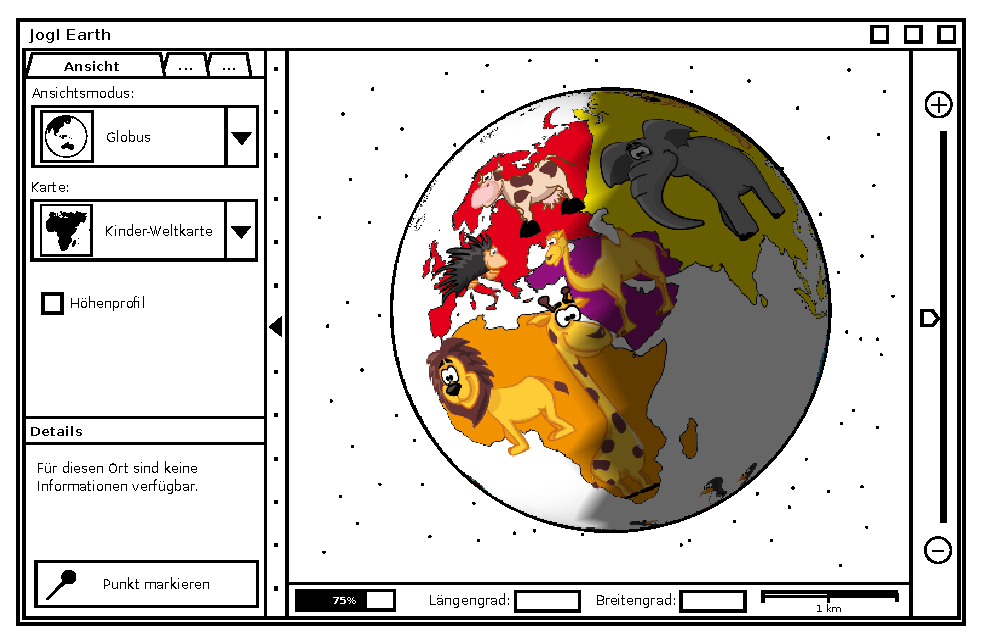
\includegraphics[scale=0.9]{GUI-Ansicht-Kinder-Weltkarte.eps}
	\caption{Die Benutzeroberfläche mit gewählter Kinder-Weltkarte}
\end{figure}
\begin{figure}
	\centering
	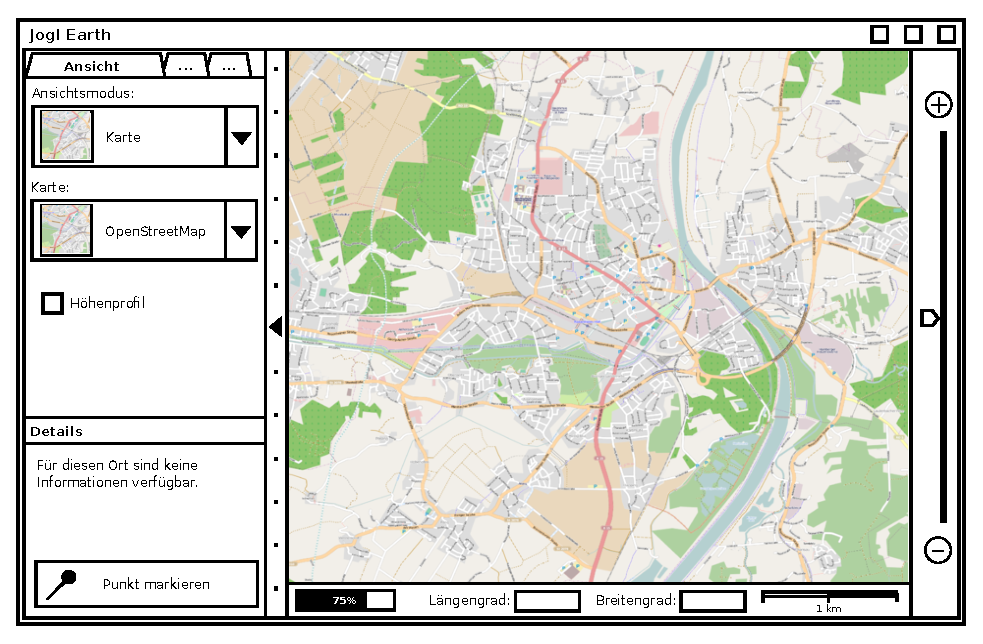
\includegraphics[scale=0.9]{GUI-Ansicht-Strassenkarte.eps}
	\caption{Die Benutzeroberfläche mit gewählter Straßenkarte}
\end{figure}

\begin{figure}
	\centering
	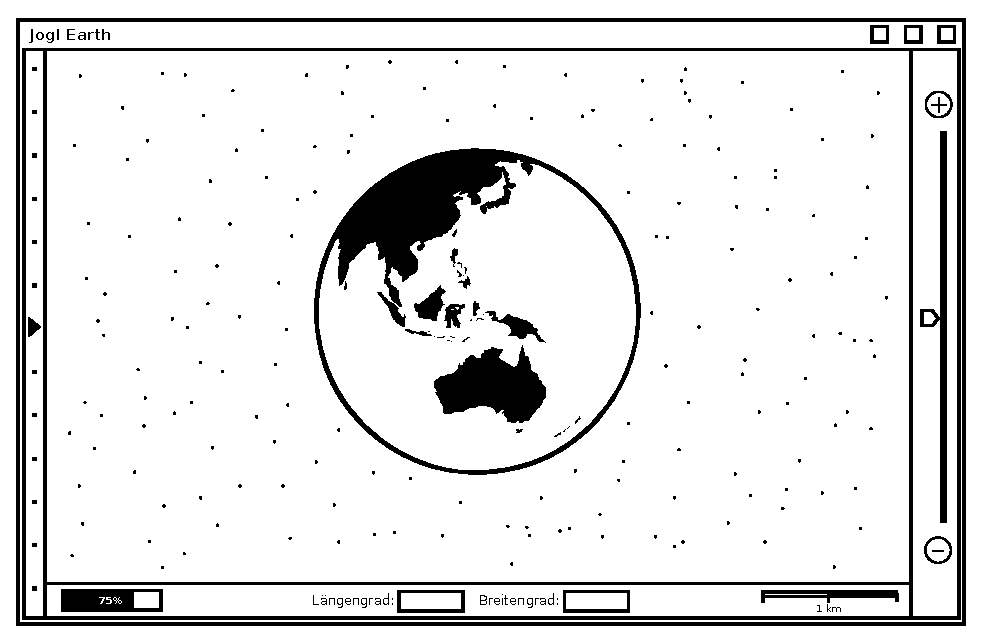
\includegraphics[scale=0.9]{GUI-Ausgeblendet.eps}
	\caption{Die Benutzeroberfläche mit ausgeblendeter Einstellungsleiste}
\end{figure}
\begin{figure}
	\centering
		\begin{minipage}[c]{6cm}
        \centering
                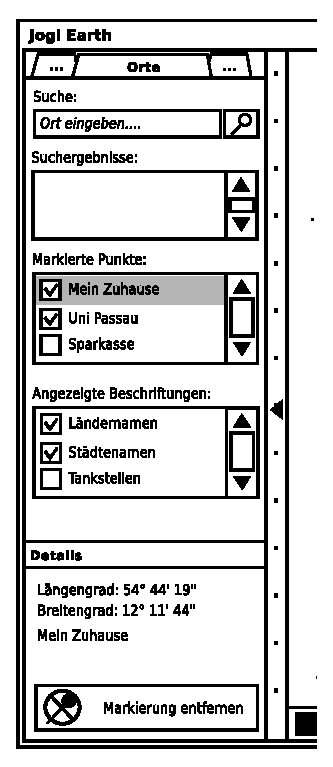
\includegraphics[scale=0.9]{GUI-Orte.eps}
        \end{minipage}
        \begin{minipage}[c]{6cm}
        \centering
                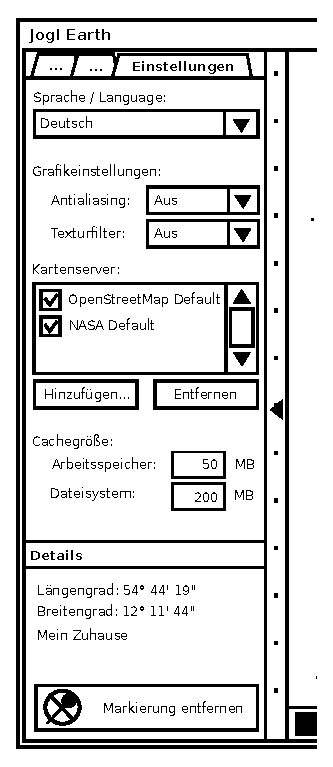
\includegraphics[scale=0.9]{GUI-Einstellungen.eps}
        \end{minipage}
        \caption{Der Orte- und der Einstellungstab}
\end{figure}
\begin{figure}
	\centering
	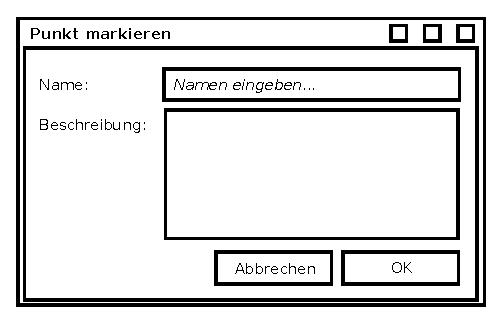
\includegraphics[scale=0.9]{GUI-Markieren.eps}
	\caption{Das Dialogfenster zum Anlegen einer neuen Markierung}
\end{figure}

\clearpage
\pagebreak

\section{Steuerung der Kartenansicht}

\vspace{3mm}
\subsection*{Mausbelegung}
\begin{tabular}{|>{\centering \arraybackslash}m{3cm}|m{9cm}|}
\hline

\includegraphics[scale=1.0]{KeyImages/mouseDrag_left.eps} & Drehen der Erdkugel / Verschieben der Karte \\ 
\hline 

\includegraphics[scale=1.0]{KeyImages/mouseDoubleClick_left.eps} & Punkt unter dem Mauszeiger im Kartenfenster zentrieren \\
\hline

\includegraphics[scale=1.0]{KeyImages/mouseDrag_right.eps} & Perspektivisches Kippen der Ansicht \\
\hline

\includegraphics[scale=1.0]{KeyImages/mouse_scrollen.eps} & Zoomen der Ansicht \\
\hline
\end{tabular} 



\vspace{5mm}
\subsection*{Tastaturbelegung}
\begin{tabular}{|>{\centering \arraybackslash}m{3cm}|m{9cm}|}
\hline
\rule[-1ex]{0pt}{7ex}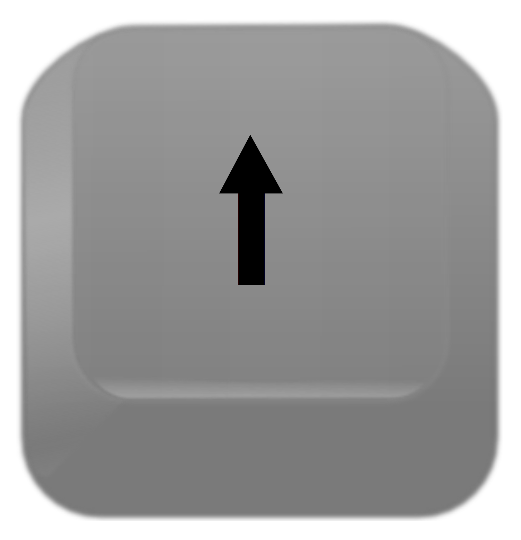
\includegraphics[scale=0.08]{KeyImages/key_arrow_up.eps}& \multirow{3}{*}{Drehen der Erdkugel / Verschieben der Karte}\\
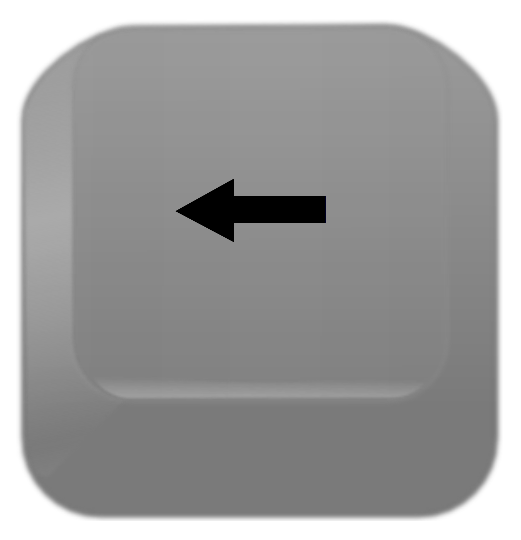
\includegraphics[scale=0.08] {KeyImages/key_arrow_left.eps} 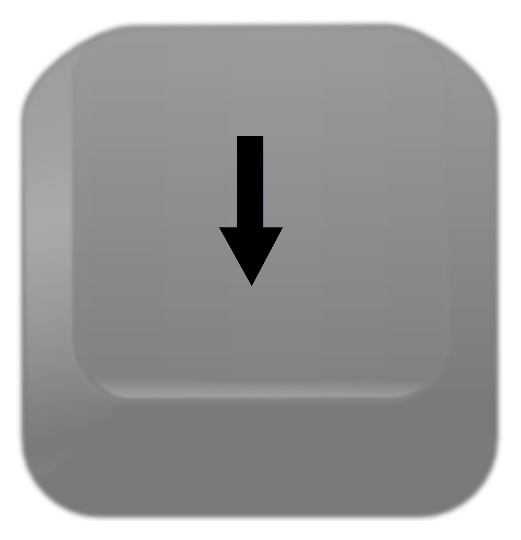
\includegraphics[scale=0.08]{KeyImages/key_arrow_down.eps} 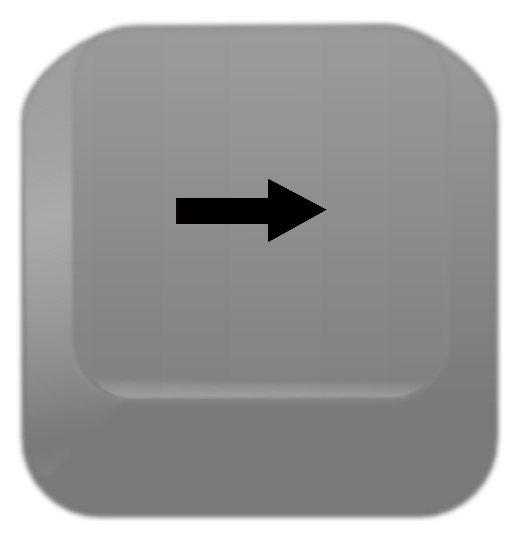
\includegraphics[scale=0.08]{KeyImages/key_arrow_right.eps} &  \\
\hline
\rule[-1ex]{0pt}{7ex} 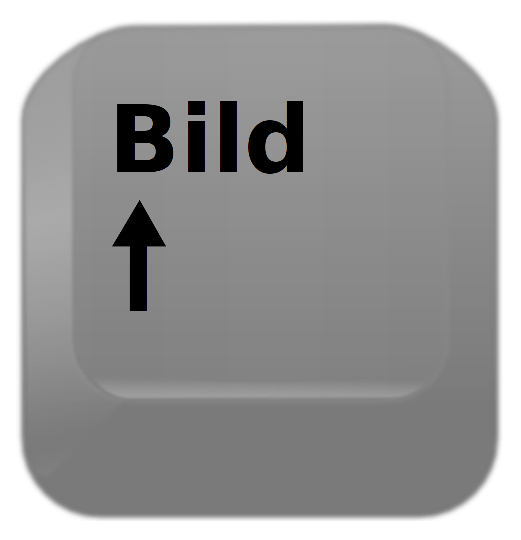
\includegraphics[scale=0.08]{KeyImages/key_Bild_Auf.eps}  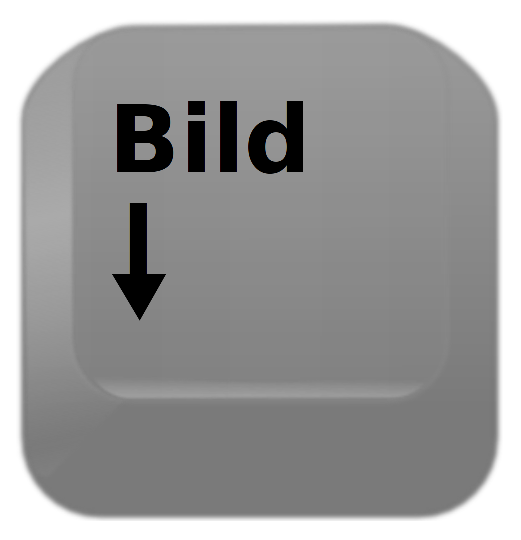
\includegraphics[scale=0.08]{KeyImages/key_Bild_Ab.eps} & Perspektivisches Kippen der Ansicht \\
\hline
\rule[-1ex]{0pt}{7ex} 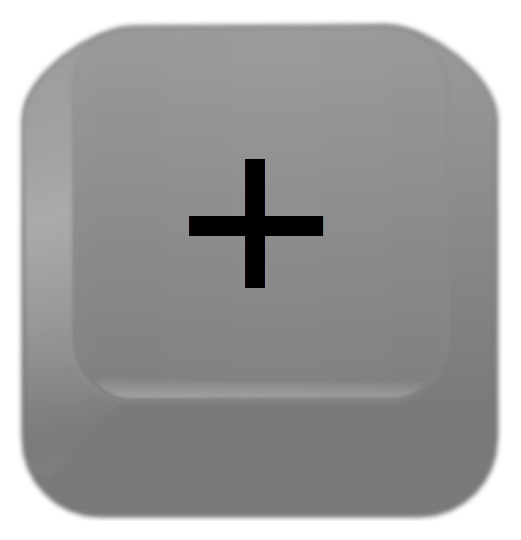
\includegraphics[scale=0.08]{KeyImages/key_Plus.eps}  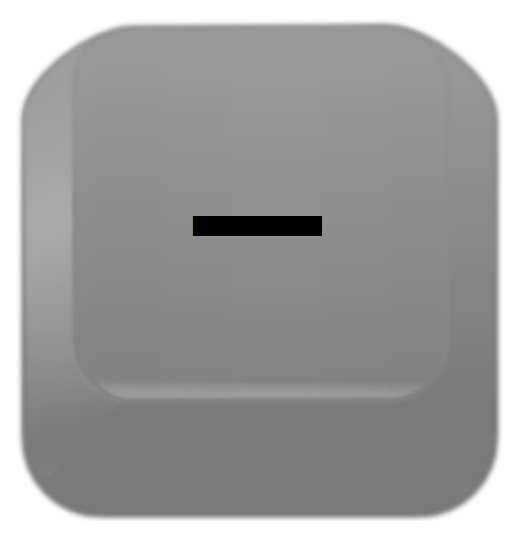
\includegraphics[scale=0.08]{KeyImages/key_Minus.eps} & Zoomen der Ansicht \\
\hline
\rule[-1ex]{0pt}{7ex} 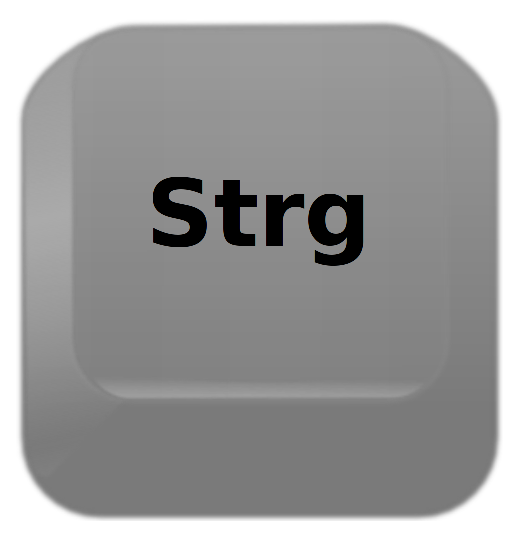
\includegraphics[scale=0.08]{KeyImages/key_Strg.eps} \rule[-1ex]{0pt}{7ex}\raisebox{0.7em}{\textbf{+}} 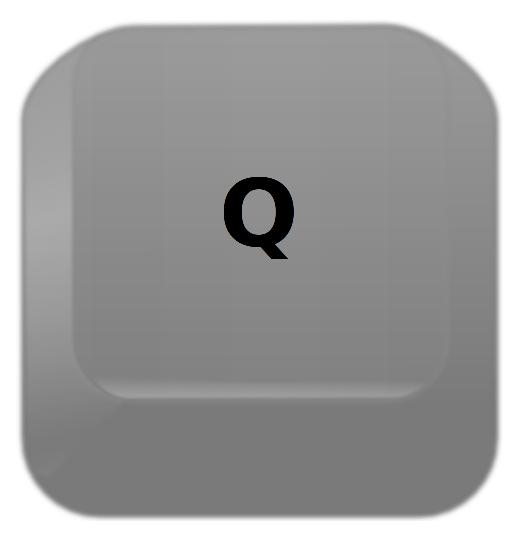
\includegraphics[scale=0.08]{KeyImages/key_Q.eps} & Beenden der Anwendung \\ 
\hline
\end{tabular} 




\chapter{Systemarchitektur}
Die Systemarchitektur folgt dem Model-View-Controller-Pattern.
\vspace{3mm}
\begin{figure}[h]
\centering
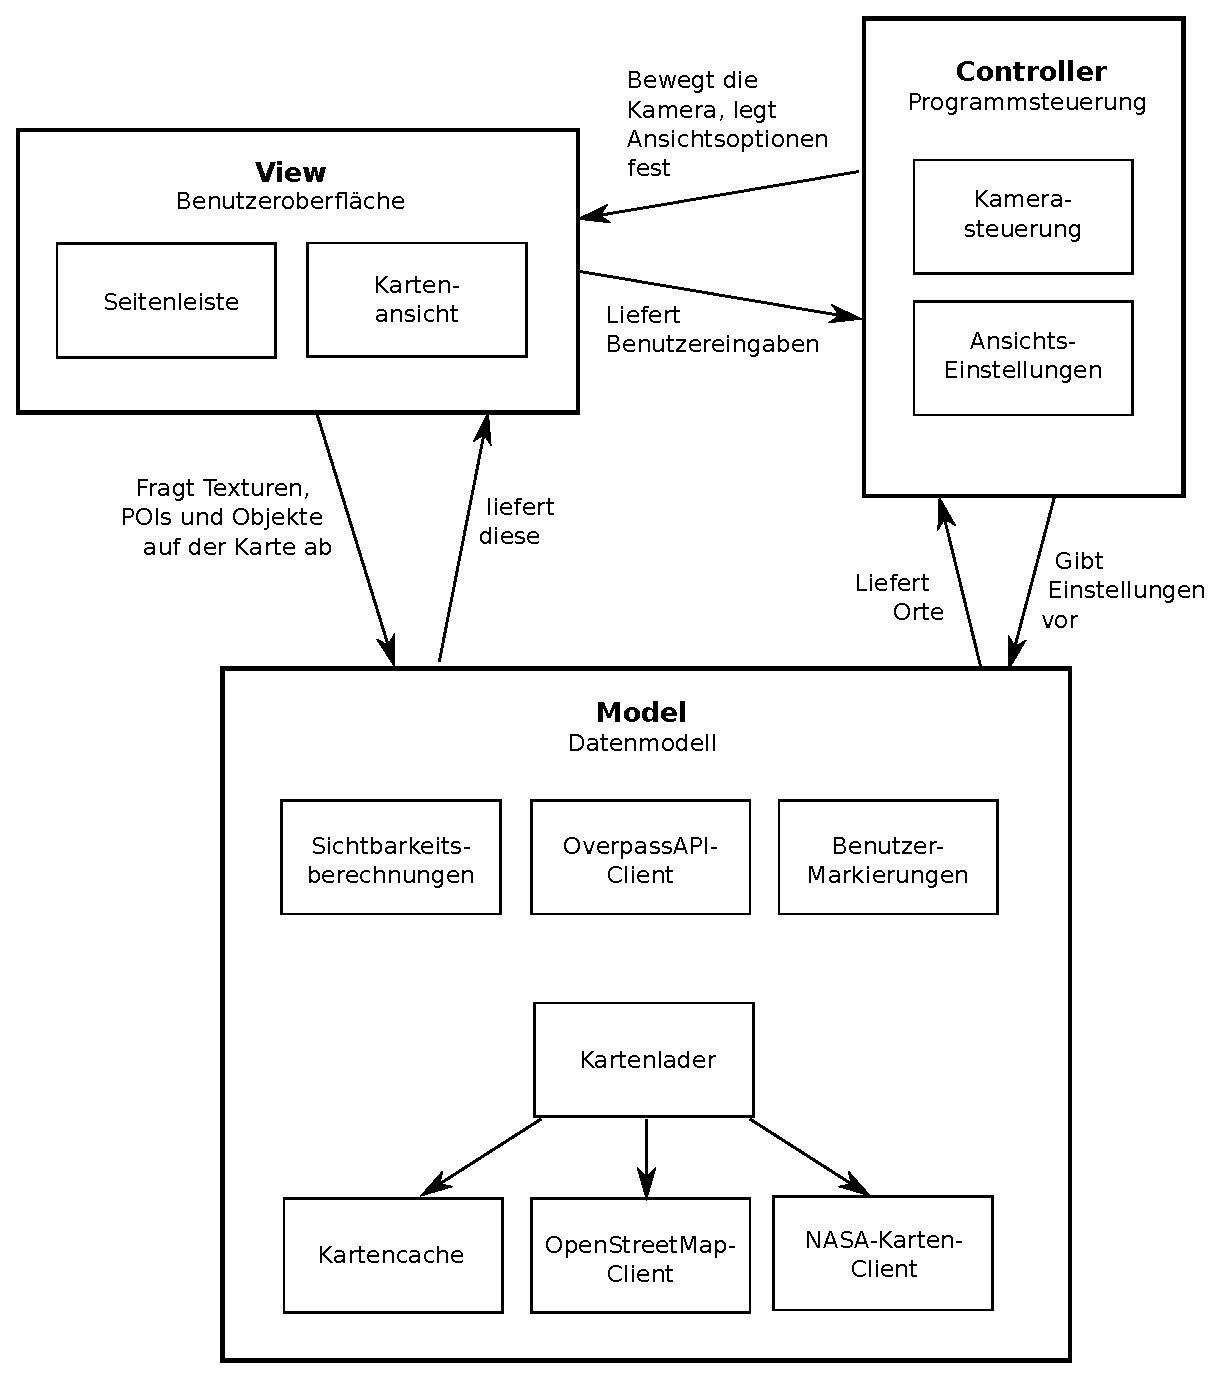
\includegraphics[scale=0.6]{ModelViewController.eps}
\caption{Konzept der Systemarchitektur (Abriss)}
\end{figure}
\subsubsection*{Controller}
Die \textbf{Programmsteuerung} übernimmt die Verarbeitung der Ein- und Ausgaben und steuert die Ansicht.
 Sie ist für die Umsetzung der Nutzerbefehle und gespeicherter Einstellungen verantwortlich.
\subsubsection*{View}
Die \textbf{Benutzeroberfläche} dient als Schnittstelle zwischen Anwender und Programm. Sie erzeugt eine visuelle Darstellung aus den Befehlen der Programmsteuerung und den Daten des Modells. Eingaben wie Tastendrücke oder das Anwählen eines GUI-Elements leitet sie an die Steuerung weiter.

\subsubsection*{Model}
Das \textbf{Datenmodell} ist dafür zuständig, Berechnungen und Anfragen bezüglich der Karte oder des Globus zu beantworten. Es bestimmt die Sichtbarkeit von Kartenabschnitten und beschafft Karten-, Markierungs- sowie ortsspezifische Daten.


\chapter{Produktfunktionen}

\nplpadding{2}
\muss
\renewcommand{\ziellabel}{F}

Wunschkriterien werden mit {\W } gekennzeichnet, alle verbleibenden sind Musskriterien.

\section{Fensterverhalten}
\begin{enumerate}[leftmargin=2.2cm]
\item Ändern der Programmfenstergröße 
\item Schließen des Fensters und damit beenden des Programms
\item Ein- und Ausklappen der Seitenleiste
\item Sprachwechsel ohne Neustart
\end{enumerate}

\section{GUI-Elemente zur Navigation}
\begin{enumerate}[leftmargin=2.2cm,resume]
\item Ändern des Zoomlevels
\item Aktualisieren der Fortschrittsanzeige für im Hintergrund geladene Daten
\item Anzeige des Längen- und Breitengrades des zentrieren Punktes.
\item Anpassen der Kameraposition durch Änderung des Längen- und Breitengrades
\item Anzeige des Benutzerhandbuchs
\item Anzeige eines Infofensters (\textit{,,About Box``})
\end{enumerate}

\section{Räumliche Berechnungen}
\begin{enumerate}[leftmargin=2.2cm,resume]
\item Erzeugung der ebenen Globusoberfläche
\item Erzeugung der Globusoberfläche aus einer Heightmap
\item Erzeugung der flachen Kartenebene
\item Erzeugung der Kartenoberfläche aus einer Heightmap
\item Berechnung des Längen- und Breitengrades unter einem Bildschirmpunkt
\item Berechnung des Maßstab des Punktes unter dem Anzeigemittelpunkt
\item Bestimmung der nötigen Kachelauflösung aus der Kameraposition
\item Entscheidung der Sichtbarkeit von Kacheln aus der Kameraposition
\wunsch
\end{enumerate}

\section{Ansichtseinstellungen}
\begin{enumerate}[leftmargin=2.2cm,resume]
\item Ändern des Ansichtsmodus
\item Ändern des Kartentyps
\wunsch
\item Zu- oder Abschalten des Höhenprofils
\item Grafikoptionen (wie Antialiasing oder Texturfilterung) sind einstellbar.
\end{enumerate}

\section{Ansichtsfenster}
\begin{enumerate}[leftmargin=2.2cm,resume]
\item Anzeige von Overlays als zweidimensionale Objekte
\item Darstellung des Sternenhimmels als Hintergrund
\end{enumerate}

\subsection{Kartenansicht}
\begin{enumerate}[leftmargin=2.2cm,resume]
\item Verschieben der Karte 
\item Kippen der Kamera relativ zu ihrer Position mit der Einschränkung, dass der Bildmittelpunkt immer auf die Karte zeigen muss
\item Verschieben der Kamera senkrecht zur Kartenebene (Zoomen) mit einer oberen und unteren Grenze
\end{enumerate}

\subsection{Globusansicht}
\begin{enumerate}[leftmargin=2.2cm,resume]
\item Drehen der Erde um ihre Achse
\item Drehen der Erde in Richtung der Pole, aber nicht über sie hinaus
\item Kippen der Kamera relativ zu ihrer Position mit der Einschränkung, dass der Bildmittelpunkt immer auf den Globus zeigen muss
\item Verschieben der Kamera senkrecht zur Globusoberfläche (Zoomen) mit einer oberen und unteren Grenze
\end{enumerate}

\section{Ortsfunktionen}
\begin{enumerate}[leftmargin=2.2cm,resume]
\item Auswahl einer begrenzten Teilmenge aus der Menge alle anzuzeigender Overlays
\wunsch
\item Markieren des Punkts am Bildmittelpunkt mit Name und Notiz
\item Entfernen eines markierten Punkts
\muss
\end{enumerate}

\section{Laden von Daten}
\begin{enumerate}[resume,leftmargin=2.2cm]
\item Hinzufügen eines Datums zu einem Cache
\item Entfernen eines Datums aus einem vollen Cache mittels einer Verdrängungsstrategie
\item Leeren des Caches
\item Ändern der zulässigen Größe eines Caches
\item Laden von Kacheln- oder Höhendaten im Hintergrund
\item Auffinden von Informationen über einen Punkt, der als Längen- und Breitengrad gegeben ist
\item Auffinden von Orten über ihren Namen
\end{enumerate}


\section{Orte}
\begin{enumerate}[leftmargin=2.2cm,resume]
\item Aktivieren und Deaktivieren eines Overlays
\wunsch
\item Anzeige von bestehenden Markierungen
\item Anzeigen und Ausblenden einer Markierung
\item Entfernen einer Markierung
\item Lokale Suche nach einem Ort im sichtbaren Kartenbereich
\item Globale Suche nach einem Ort
\item Anzeige von Suchergebnissen
\end{enumerate}


\chapter{Produktdaten}

\renewcommand{\ziellabel}{D}
\muss

Wunschkriterien werden mit {\W } gekennzeichnet, alle verbleibenden sind Musskriterien.\\

\vspace{5mm}

\begin{enumerate}[leftmargin=2cm]
\item Alle Daten des Programms werden im Verzeichnis der JAR-Datei (oder falls extra angegeben in einem Unterordner) abgelegt.
\item Es werden alle benötigten Bibliotheken mitgeliefert, das sind im einzelnen: 
\begin{itemize}
\item JOGL mit allen betriebssystemabhängigen Bibliotheken
\item die Forms-Bibliothek von JGoodies.
\end{itemize}
\wunsch
\item Einstellungen werden in einer Datei \texttt{settings} gespeichert, die mit den Vorgabeeinstellungen dem Programm beiliegt. Zu den gespeicherten Daten gehören:
\begin{itemize}
\item Sprache
\item Antialiasing und Texturfilter
\item die verfügbaren und momentan gewählten Kartenserver
\item eingestellte Puffergrößen
\item der zuletzt ausgewählte Ansichtsmodus, die gewählte Karte, Overlays und Ansichtsoptionen wie 3D-Modelle
\item markierte Punkte mit Name und Notiz
\end{itemize}
\muss
\item Mitgelieferte Texturen wie beispielsweise die Kinder-Weltkarte oder Symbole für POIs liegen im Ordner \texttt{textures}.
\begin{figure}[!htb]
	\centering
	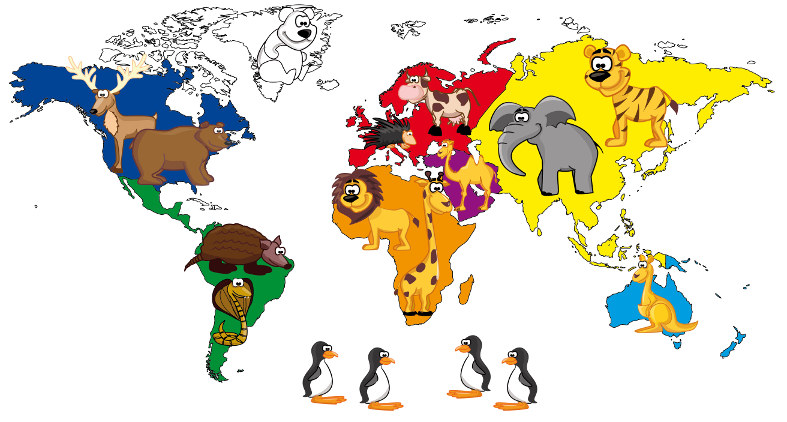
\includegraphics[scale=0.3]{Kinder-Weltkarte.jpg}
\end{figure}
\item Zwischengespeicherte Kacheln werden im Ordner \texttt{cache} abgelegt. Dabei erhält jede Kombination aus Server- und Kartentyp ein eigenes Unterverzeichnis.
\end{enumerate}


\chapter{Produktleistungen}

\renewcommand{\ziellabel}{L}
\muss

Wunschkriterien werden mit {\W } gekennzeichnet, alle verbleibenden sind Musskriterien.

\begin{enumerate}[leftmargin=2.2cm]
\item Die Benutzeroberfläche ist grafisch ansprechend, gut strukturiert und intuitiv verständlich gehalten.
\wunsch
\item Um auch Kinder zu motivieren, \JoglEarth zu verwenden, wird eine altersgemäße Kinder-Weltkarte mit ausgeliefert.
\muss
\item Die Oberfläche wird in den Sprachen Englisch und Deutsch angeboten.
\item Die gesamte GUI ist komfortabel mit Maus und Tastatur steuerbar.
\item Die einklappbare Seitenleiste in der GUI soll dem Benutzer die Möglichkeit bieten, 3D- und 2D-Ansichten in einem größeren Umfang (flächig) darzustellen.
\item Die Bewegung der Kamera und das Anpassen des Zoomlevels wird beschränkt, damit keine Darstellungsfehler wie das Durchdringen der Kartenebene auftreten.
\item Die Menge der angezeigten Overlays und 3D-Modelle wird beschränkt, sodass die Leistung wie auch die Lesbarkeit von Beschriftungen gegeben ist.
\item Eine weitere Option für den Benutzer soll das Markieren von Punkten bzw. Orten in den Karten darstellen. Diese sollen gespeichert und mit Namen und Notizen versehen werden können.
\item Zudem soll eine Suchfunktion den Nutzer unterstützen, die POIs oder Städte/ Orte unkompliziert aufzufinden. Dies geschieht unabhängig von der Sprache des eingetippten Suchbegriffs.
\item Kartendaten werden effizient zwischengespeichert, um sowohl unnötiges Nachladen als auch den Speicherverbrauch zu minimieren.
\item Hintergrundvorgänge des Programms wie das Nachladen von Kartendaten unterbrechen den Rendervorgang nicht.
\item Ein Ladebalken verdeutlicht den Status der im Hintergrund geladenen Kartenkacheln.
\item Nicht verfügbare Kartenausschnitte sollen durch eine Platzhaltertextur ersetzt werden.
\wunsch
\item Rendervorgänge sollen nur bei Bildänderungen gestartet werden und minimieren somit den Energieverbrauch.
\item Die Anwendung ist intuitiv mit der Toucheingabe auf Windows 8 bedienbar.
\item Die Grafikeinstellungen lassen sich anpassen, sodass die Leistung auch auf älterer Hardware akzeptabel ist.
\item Mit zusätzlichen Darstellungsmöglichkeiten, wie 3D-Höhenprofile, eine Sonnensystem-Modellansicht und einem Sternenhimmel als Hintergrundmotiv werden die Ansichten optisch aufgewertet.
\end{enumerate}



\chapter{Qualitätsbestimmungen}


\vspace{1cm}
\begin{center}
\begin{tabular}{lcccc}
\hline 
\rule[-1ex]{0pt}{4ex} \textit{Produktqualität} & \textit{sehr gut} & \textit{gut} & \textit{normal} & \textit{nicht relevant} \\ 
\hline 
\rule[-1ex]{0pt}{4ex} \textbf{Funktionalität} &  &  &  &  \\ 
\rule[-1ex]{0pt}{4ex} \hspace{10pt} Web-Mining & &  & • & \\ 
\rule[-1ex]{0pt}{4ex} \hspace{10pt} Interoperabilität & & • & & \\ 

\hline 
\rule[-1ex]{0pt}{4ex} \textbf{Zuverlässigkeit} &  &  &  &  \\ 
\rule[-1ex]{0pt}{4ex} \hspace{10pt} Stabilität & • & & & \\ 
\rule[-1ex]{0pt}{4ex} \hspace{10pt} Fehlertoleranz & • & & & \\ 
\rule[-1ex]{0pt}{4ex} \hspace{10pt} Wiederherstellbarkeit &  &  &  & • \\ 

\hline 
\rule[-1ex]{0pt}{4ex} \textbf{Benutzbarkeit} &  &  &  &  \\ 
\rule[-1ex]{0pt}{4ex} \hspace{10pt} Bedienbarkeit & • & & & \\ 
\rule[-1ex]{0pt}{4ex} \hspace{10pt} Erlernbarkeit & • & & & \\ 
\rule[-1ex]{0pt}{4ex} \hspace{10pt} Grafische Gestaltung & & • & & \\ 
\rule[-1ex]{0pt}{4ex} \hspace{10pt} Verständlichkeit & • & & & \\ 

\hline 
\rule[-1ex]{0pt}{4ex} \textbf{Effizienz} &  &  &  &  \\ 
\rule[-1ex]{0pt}{4ex} \hspace{10pt} Bildqualität & & • & & \\ 
\rule[-1ex]{0pt}{4ex} \hspace{10pt} Laufzeit & & • & & \\ 
\rule[-1ex]{0pt}{4ex} \hspace{10pt} Speichermanagement & • & & & \\ 

\hline 
\rule[-1ex]{0pt}{4ex} \textbf{Anpassfähigkeit} &  &  &  &  \\ 
\rule[-1ex]{0pt}{4ex} \hspace{10pt} Code-Qualität & & • & & \\ 
\rule[-1ex]{0pt}{4ex} \hspace{10pt} Modifizierbarkeit & & & • & \\ 

\hline 
\rule[-1ex]{0pt}{4ex} \textbf{Portierbarkeit} &  &  &  &  \\ 
\rule[-1ex]{0pt}{4ex} \hspace{10pt} Erweiterbarkeit & & & • & \\ 
\rule[-1ex]{0pt}{4ex} \hspace{10pt} Konformität & & • & & \\ 

\hline 
\rule[-1ex]{0pt}{4ex} \textbf{Dokumentation} & • & & & \\ 
\hline 
\end{tabular} 
\end{center}

\pagebreak



\section*{Funktionalität}
\begin{details}
\item \sfbf{Web Mining:} Automatische Extraktion von Daten aus dem Internet. Bei \JoglEarth findet das Web Mining bei der Suchfunktion Anwendung. Um die Benutzeroberfläche übersichtlich zu halten, ist nur eine einfache Suche nach Wortteilen möglich, die nicht weiter eingegrenzt wird. Es wird weiter vorausgesetzt, dass sich die Overpass-Server genau wie in der Spezifikation verhalten; eine Fehlerkorrektur wird nicht versucht.

\item \textbf{Interoperabilität:} Die Anwendung soll mit OpenStreetMap, der Overpass-API und ähnlichen Diensten interagieren um das Kartenmaterial mit Zusatzinformationen grafisch zu unterstützen. Da dies Kernbestandteil ist, wird Wert auf die Qualität der Interoperabilität gelegt.
\end{details}


\section*{Zuverlässigkeit}
\begin{details}
\item \sfbf{Stabilität:} Die Lauffähigkeit des Programms soll nicht unterbrochen bzw. beeinträchtigt werden. Programmabstürze und Fehlverhalten führt sehr schnell zu Unzufriedenheit beim Benutzer, weswegen der Stabilität hohe Priorität zukommt.

\item \sfbf{Fehlertoleranz:} Das Programm soll trotz fehlerhafter Eingaben seitens des Anwenders seine Funktionsweise aufrechterhalten. Dies ist ein wichtiger Punkt, da falsche Behandlung von unsinnigen Eingaben zu Fehlverhalten führt (siehe Stabilität).

\item \sfbf{Wiederherstellbarkeit:} Bei Neustart nach unsachgemäßer Beendigung des Programms, z.B. durch einen Systemabsturz, verhält sich das Programm wie bei einem normalen Start. Es wird kein Versuch unternommen, die Sitzung wiederherzustellen, da der Zustand keine Informationen enthält, die für den Benutzer kritisch sind.
\end{details}


\section*{Benutzbarkeit}
\begin{details}
\item \sfbf{Bedienbarkeit:} Die Oberfläche soll intuitiv bedienbar sein. Dies ist auch deshalb von Bedeutung, da Kinder zur Zielgruppe gehören.

\item \sfbf{Erlernbarkeit:} Die Bedienung der Oberfläche soll einfach verstanden werden. Dies deckt sich mit der Anforderung nach intuitiver Bedienbarkeit.

\item \sfbf{Grafische Gestaltung:} Die Oberfläche soll optisch ansprechend wirken. Dabei wird auch auf Einfachheit geachtet, was der Erlernbarkeit dient.

\item \sfbf{Verständlichkeit:} Die Oberfläche soll selbsterklärend sein. Dieses Ziel ist leicht erreichbar, da der Funktionsumfang gut strukturiert ist.
\end{details}


\section*{Effizienz}
\begin{details}
\item \sfbf{Bildqualität:} Die Satellitenbilder und Kartendaten sollen in bestmöglicher Qualität dargestellt werden, außerdem sollen Bildänderungen flüssig erfolgen. Dies ist für die Sichtbarkeit von Kartendetails und die Bedienbarkeit unabdinglich.

\item \sfbf{Laufzeit:} Trotz bestmöglicher Bildqualität sollen die Wartezeiten zum Laden der Daten gering gehalten werden. Die Zielsetzung ist es, dabei heutige Standards zu erreichen.

\item \sfbf{Speichermanagement:} Die Kachel-Daten werden im Dateisystem und im Arbeitsspeicher effizient gepuffert. Effizientes Speichermanagement wirkt sich unmittelbar auf die Ladezeiten aus, weswegen es höchste Aufmerksamkeit genießt.
\end{details}


\section*{Anpassfähigkeit}
\begin{details}
\item \sfbf{Code-Qualität:} Der Quellcode des Programms soll leicht verständlich gehalten werden. Dies ist für die Teamarbeit unerlässlich.

\item \sfbf{Modifizierbarkeit:} Zusätzliche Änderungen bzw. Anpassungen des Codes sollen einfach umsetzbar sein. Da die Software nach Beendigung des Projekts nicht weiterentwickelt wird, spielt dies eine untergeordnete Rolle.
\end{details}


\section*{Portierbarkeit}
\begin{details}
\item \sfbf{Erweiterbarkeit:} Zusätzliche Funktionalitäten sollen in den Code integrierbar sein. Hier gilt das selbe wie für die Modifizierbarkeit.

\item \sfbf{Konformität:} Vorgegebene Konventionen sollen eingehalten werden. 
\end{details}


\section*{Dokumentation}
\begin{details}
\item \sfbf{Dokumentation:} Ein gutes Softwareprodukt zeichnet sich unter Anderem durch die Qualität des Benutzerhandbuchs, der Quelltextdokumentation, der einzelnen Phasendokumente aus. Sie sollen gut strukturiert, leicht verständlich und fachlich kompetent gehalten sein. 
\end{details}




\chapter{Globale Testszenarien und Testfälle}

\renewcommand{\ziellabel}{T}

\begin{details}[2pt]
\item \sfbf{Ausgangspunkt:} Nackte Grundinstallation 
\item \sfbf{Test:} Szenario - Anwendungsstart 
\item \sfbf{Voraussetzung:} keine
\end{details}
\vspace{2mm}
\begin{enumerate}[leftmargin = 2.2cm]
\item Das Programm wird gestartet. Es öffnet sich die GUI in Standardgröße (1024x768 Pixeln) (siehe \ziel{F010}).
\item Die Einstellungsleiste der GUI ist geöffnet (siehe \ziel{F030}).
\item Die GUI startet in Standardsprache Deutsch (siehe \ziel{F040}).
\wunsch
\item Die GUI startet im Sonnensystemmodus. Erneute Auswahl des Sonnensystemmodus darf nicht mehr möglich sein. Die Auswahl des Kartentyps, Höhenprofil und 3D-Modelle muss entfallen (gemäß Abbildung 5.1) (siehe \ziel{F100W}, \ziel{F130W}).
\muss
\item Sollte der (\W) Sonnensystemmodus nicht realisiert werden, startet die GUI in der Globus-Ansicht mit Satellitenbildern. Erneute Auswahl des Ansichtsmodus Globus mit Satellitenbildern darf nicht mehr möglich sein (siehe \ziel{F090}, \ziel{F110}).
\end{enumerate}

\vspace{1.0cm}
\begin{details}[2pt]
\item \sfbf{Ausgangspunkt:} Nackte Grundinstallation 
\item \sfbf{Test:} Funktionalität GUI inklusive der gelieferten Texturen 
\item \sfbf{Voraussetzung:} Szenario - Anwendungsstart ausführen
\end{details}
\vspace{2mm}
\begin{enumerate}[leftmargin = 2.2cm, resume]
\item Änderung der Sprache auf Englisch - die Anzeigesprache ändert sich - Rücksetzen der Sprache auf Deutsch (siehe \ziel{F040}).
\item Maßstabsanzeige betrachten und Skalierung notieren (siehe \ziel{F080}).
\item Zoomlevel - Augangspunkt notieren, dann Zoomlevel erhöhen und Maßstabsänderung kontrollieren (siehe \ziel{F050}, \ziel{F080}).
\item Maximales und Minimales Zoomlevel einstellen - Ansicht passt sich an (siehe \ziel{F210}).
\item Zoomlevel verringern und Maßstabsänderung kontrollieren (siehe \ziel{F050}, \ziel{F080}).
\item Zoomlevel wieder rücksetzen auf Ausgangspunkt (siehe \ziel{F050}).
\item Maßstabsanzeige vergleichen mit vorheriger Skalierung (siehe \ziel{F080}).
\wunsch
\item Höhenprofile einschalten und anschließend wieder ausschalten (siehe \ziel{F120W}).
\item 3D-Modelle für Häuse/Bäume einschalten und anschließend wieder ausschalten (siehe \ziel{F120W}, \ziel{F230W}).
\item Grafikeinstellung - Antialiasing einschalten und anschließend wieder ausschalten (siehe \ziel{F150W}).
\item Grafikeinstellung - Texturfilterung einschalten und anschließend wieder ausschalten (siehe \ziel{F150W}).
\muss
\item Steuerung mittels Maus: Erde über die Pole drehen über X-Achse. Erde dreht sich konsistent - Pole dürfen sich jedoch nur $+/- 90^\circ$ drehen lassen - Pole wieder zurück drehen (siehe \ziel{F160}, \ziel{F180}, \ziel{F210}).
\item Steuerung mittels Maus: Erde über die Pole drehen über Y-Achse. Erde dreht sich konsistent - Pole dürfen sich jedoch nur $+/- 90^\circ$ drehen lassen - Pole wieder zurück drehen (siehe \ziel{F160}, \ziel{F180}, \ziel{F210}).
\item Steuerung mittels Tastatur: Erde über die Pole drehen über X-Achse. Erde dreht sich konsistent - Pole dürfen sich jedoch nur $+/- 90^\circ$ drehen lassen - Pole wieder zurück drehen (siehe \ziel{F160}, \ziel{F180}, \ziel{F210}).
\item Steuerung mittels Tastatur: Erde über die Pole drehen über Y-Achse. Erde dreht sich konsistent - Pole dürfen sich jedoch nur $+/- 90^\circ$ drehen lassen - Pole wieder zurück drehen (siehe \ziel{F160}, \ziel{F180}, \ziel{F210}).
\item Eingabe von gültigen Längen- oder Breitengraden. Der Globus richtet sich entsprechend aus und zentriert den Punkt (siehe \ziel{F070}).
\item Eingabe von ungültigen Längen- oder Breitengraden. Die Ansicht verändert sich nicht (siehe \ziel{F070}).
\item Ausblenden der Seitenleiste (siehe \ziel{F030}).
\item Einblenden der Seitenleiste (siehe \ziel{F030}).
\wunsch
\item Auswahl der Kinder-Weltkarte - Ansicht ändert sich entsprechend. Erneute Auswahl des Globus mit Kinder-Weltkarte darf nicht mehr möglich sein (siehe \ziel{F100W}).
\item Sternenhimmel als Hintergrundbild einschalten und anschließend wieder ausschalten (siehe \ziel{F140W}).
\muss
\item Globus kippen und wieder Rücksetzen (siehe \ziel{F180}).
\item Verkleinern des Fensters - Minimalgröße (800x600 Pixel) darf nicht unterschritten werden (siehe \ziel{F010}).
\item Schließen der Anwendung mit Strg + Q ohne Rückmeldung (siehe \ziel{F020}).
\end{enumerate}

\vspace{1.0cm}
\begin{details}[2pt]
\item \sfbf{Ausgangspunkt:} Nackte Grundinstallation \\
\item \sfbf{Test:} Laden der Kartendaten von OpenStreetMap und NASA \\
\item \sfbf{Voraussetzung:} Szenario - Anwendungsstart ausführen
\end{details}
\vspace{2mm}
\begin{enumerate}[leftmargin = 2.2cm, resume]
\item Laden der Kartenkacheln testen (siehe \ziel{F250}, \ziel{F260}, \ziel{F270}, \ziel{F290}, \ziel{F300}).
\wunsch
\item Kontrollieren, ob Platzhaltertextur während des Ladens der Kartenkacheln erscheint (siehe \ziel{F310W}).
\item Die Kacheln der direkten Randbereiche außerhalb der Ansicht werden geladen (siehe \ziel{F320W}).
\item Ist die Textur einer Kachel noch nicht geladen, wird zuerst versucht sie aus dem Cache im Arbeitsspeicher, dann aus dem Cache im Dateisystem zu laden (siehe \ziel{F330W}).
\muss
\item Ladebalken für Fortschritt beobachten (siehe \ziel{F060}).
\item Wenn Ladebalken 100\% erreicht hat, wird die Kachel direkt angezeigt (siehe \ziel{F060}, \ziel{F280}).
\item Drücken des Schließen-Buttons beendet die Anwendung ohne Rückmeldung. Die Einstellungen der Kartendaten müssen hier gespeichert werden (siehe \ziel{F020}).
\end{enumerate}

\vspace{1.0cm}
\begin{details}[2pt]
\item \sfbf{Ausgangspunkt:} Geladene Kartendaten 
\item \sfbf{Test:} Ansichtseinstellungen bei Karten 
\item \sfbf{Voraussetzung:} Szenario - Anwendungsstart ausführen
\end{details}
\begin{enumerate}[leftmargin = 2.2cm, resume]
\item Auswahl der Ansicht Karte mit Kartentyp OpenStreetMap (Straßenkarte) (siehe \ziel{F090}, \ziel{F110}).
\wunsch
\item Höhenprofile einschalten und anschließend wieder ausschalten (siehe \ziel{F120W}).
\item 3D-Modelle für Häuse/Bäume einschalten und anschließend wieder ausschalten (siehe \ziel{F120W}, \ziel{F230W}).
\item Grafikeinstellung - Antialiasing einschalten und anschließend wieder ausschalten (siehe \ziel{F150W}).
\item Grafikeinstellung - Texturfilterung einschalten und anschließend wieder ausschalten (siehe \ziel{F150W}).
\muss
\item Verschieben der Karten: Ansicht nach links/rechts/oben/unten verändern (siehe \ziel{F170}).
\item Kippen des Kartenausschnitts und wieder Rücksetzen (siehe \ziel{F170}).
\item Schließen der Anwendung mit Strg + Q ohne Rückmeldung (siehe \ziel{F020}).
\end{enumerate}


\vspace{1.0cm}
\begin{details}[2pt]
\item \sfbf{Ausgangspunkt:} Geladene Kartendaten 
\item \sfbf{Test:} Punkte markieren, POIs 
\item \sfbf{Voraussetzung:} Szenario - Anwendungsstart ausführen
\end{details}
\vspace{2mm}
\begin{enumerate}[leftmargin = 2.2cm, resume]
\item Auswahl der Ansicht Karte mit Kartentyp OpenStreetMap (Straßenkarte) (siehe \ziel{F090}, \ziel{F110}).
\item Im Detailfenster müssen Informationen zum zentrierten Punkt, wie Längen- und Breitengrad angezeigt werden (siehe \ziel{F200}, \ziel{F380})
\wunsch
\item Suche mehrerer Orte/ Punkte auf Karten mittels Suchfunktion. Suchergebnisse müssen angezeigt werden (siehe \ziel{F370W}).
\item Button Punkt markieren klicken und Punkt auf der Karte markieren. Der markierte Punkt wird nun im Kartenfenster zentriert (siehe \ziel{F190W}, \ziel{F230W}).
\item Im Detailfenster müssen Informationen zum markierten Punkt, wie Längen- und Breitengrad angezeigt werden (siehe \ziel{F200}).
\item Markierung des Punkts aus-/einblenden (siehe \ziel{F360W}).
\item Markierten Punkt in der Liste speichern. Name und Bezeichnung eintragen (siehe \ziel{F360W}, \ziel{F390W}, \ziel{F400W}).
\item Button Punkt markieren klicken und zweiten Punkt auf der Karte markieren. Der markierte Punkt wird nun im Kartenfenster zentriert (siehe \ziel{F190W}, \ziel{F230W}).
\item Im Detailfenster müssen Informationen zum neuen markierten Punkt, wie Längen- und Breitengrad angezeigt werden (siehe \ziel{F200}).
\item Markierten Punkt in der Liste speichern. Name und Bezeichnung eintragen (siehe \ziel{F360W}, \ziel{F390W}, \ziel{F400W}).
\item Button Punkt markieren klicken und dritten Punkt auf der Karte markieren. Der markierte Punkt wird nun im Kartenfenster zentriert (siehe \ziel{F190W}, \ziel{F230W}).
\item Markierten Punkt in der Liste speichern. Name und Bezeichnung eintragen (siehe \ziel{F360W}, \ziel{F390W}, \ziel{F400W}).
\item Gespeicherten Punkt '2' aus der Liste löschen ohne Rückmeldung (siehe \ziel{F360W}, \ziel{F390W}, \ziel{F400W}).
\item Markierten Punkt '1' und Punkt '3' in der Liste speichern (siehe \ziel{F360W}, \ziel{F390W}, \ziel{F400W}).
\muss
\item Anzeige von Overlays, wie Städtenamen anwählen (siehe \ziel{F220}, \ziel{F350}).
\item Anzeige von POIs, wie Tankstellen anwählen (siehe \ziel{F220}, \ziel{F350}).
\item Alle Overlays anwählen - Testen ob Lesbarkeit der Beschriftungen und der Symbole gegeben ist. Anschließend alle Overlays abwählen (siehe \ziel{F220}, \ziel{F240}).
\item 3D-Modelle zuschalten - Testen ob Lesbarkeit der Beschriftungen und der Symbole gegeben ist (siehe \ziel{F240}).
\item  Schließen der Anwendung mit Strg + Q ohne Rückmeldung. Die Einstellungen der Kartendaten und der markierten Punkte müssen hier gespeichert werden (siehe \ziel{F020}).
\end{enumerate}

\vspace{1.0cm}
\begin{details}[2pt]
\item \sfbf{Ausgangspunkt:} Liste der markierten Punkte und die Ansichtseinstellungen werden übernommen
\item \sfbf{Test:} Settings Speicherung
\item \sfbf{Voraussetzung:} Szenario - Anwendungsstart ausführen, Veränderung der Settings-Datei (z.B. markierte Punkte setzen)
\end{details}
\vspace{2mm}
\begin{enumerate}[leftmargin = 2.2cm, resume]
\wunsch
\item Kontrolle ob die Settings-Einstellungen übernommen wurden. (siehe \ziel{F390W}, \ziel{F400W})
\item Kontrolle ob die beiden markierten Punkte noch in der Liste vorhanden sind (siehe \ziel{F360W}, \ziel{F390W}, \ziel{F400W}).
\item Cache-Größen mehrmals verändern (siehe \ziel{F330W}).
\muss
\item Drücken des Schließen-Buttons beendet die Anwendung ohne Rückmeldung. (siehe \ziel{F020})
\end{enumerate}



\chapter{Entwicklungsumgebung}
\section{Software}
Abgesehen vom Betriebssystem und Anwendungen wie Texteditoren ist die verwendete Software im Entwicklerteam einheitlich.
\begin{itemize}
\item Betriebssysteme: Windows 7, Windows 8, Linux, jeweils auf x86{\_}64
\item Entwicklungsumgebung: Eclipse
\item Framework: Java 7 (JDK)
\item Unit Tests: JUnit
\item Messtool zur Testabdeckung: EclEmma
\item Bugtracking: Mit Github
\item Grafik- und Bildbearbeitung: Inkscape, GIMP
\item Textsatz: \LaTeX
\item Versionsverwaltung: Git mit Repository bei GitHub
\item Visualisierung: IBM Software Rational Architect, Microsoft Visio
\item Teamkommunikation: E-Mail
\end{itemize}

\vspace{5mm}
\section{Hardware}
Auch wenn die Hardwareanforderungen bereits gegeben sind, sei hier einmal die Ausstattung der Entwickler aufgeführt um die genauen Testbedingungen zu formulieren.

\vspace{0.5cm}

\begin{tabular}{|l|c|c|c|}
\hline
\rule[-1ex]{0pt}{4ex}\textsf{\textbf{Entwickler}} & \textsf{\textbf{Prozessor}} & \textsf{\textbf{RAM}} & \textsf{\textbf{Grafik}} \\
\hline
\hline
\rule[-1ex]{0pt}{4ex}\multirow{2}{*}{Fabian Knorr} & AMD PhenomII X4 840 @3,2GHz & 8 GB & ATi Radeon HD 6850 \\
\rule[-1ex]{0pt}{2ex} & AMD Athlon Neo X2 L335 @1,6GHz & 4 GB & ATi Radeon HD 3200 \\
\hline
\rule[-1ex]{0pt}{4ex}Gabriele Haas & Intel Core i3 550 @3,2GHz & 4 GB & Intel HD Graphics (i3) \\
\hline
\rule[-1ex]{0pt}{4ex}Christof Blauberger & AMD A6-3420M & 8 GB & ATi Radeon HD 6520/7470M \\
\hline
\rule[-1ex]{0pt}{4ex}Constantin Wenger & Intel i7-3770K @3.50GHz & 24GB & Nvidia GTX 770 4GB \\
\hline
\rule[-1ex]{0pt}{4ex}Thomas Eder & AMD A4-3400 & 8 GB & Nvidia GTX 260 \\
\hline
\rule[-1ex]{0pt}{4ex}\multirow{2}{*}{Sebastian Reichl} & AMD PhenomII X6 1100T @3,4Ghz & 8 GB & ATI Radeon HD 6950 \\
\rule[-1ex]{0pt}{2ex}& Intel Core i5-4200U @ 2,29 Ghz & 4 GB & Intel HD Graphics \\
\hline
\end{tabular}


\chapter*{Glossar}
\addcontentsline{toc}{chapter}{Glossar}
\newcolumntype{L}[1]{>{\sffamily\bfseries\hsize=#1\hsize\raggedright\arraybackslash}X}
\newcolumntype{R}[1]{>{\hsize=#1\hsize\raggedright\arraybackslash}X}
\setlength{\extrarowheight}{4mm}
\begin{longtabu}{L{0.35} R{1.65}}
Anisotropes Filtern & Methode um den Schärfeeindruck von perspektivisch verzerrten \textref{Texturen} zu verbessern\\
Antialiasing & Methode zur Kantenglättung beim \textref{Rendern}\\
API & (Application Programming Interface) Programmierschnittstelle zu einer Programmbibliothek oder einem Dienst\\
Bildauflösung & Breite und Höhe einer Grafik in Pixel, umgangssprachlich auch deren Produkt (,,Megapixel``) \\
Bildkachel & Element einer rasterförmigen Zerteilung eines (für den Anwendungszweck zu großen) Bildes\\
BSD-Lizenz & (Berkeley Software Distribution-Lizenz) Gruppe von Lizenzen aus dem \textref{Open-Source}-Bereich.\\
Cache & \textref{Pufferspeicher}\\
Client & (Netzwerktechnik) Knoten eines Netzwerks, die den Dienst eines \textref{Servers} nutzt. Für gewöhnlich eine Anwendung auf Benutzerseite.\\
EclEmma & Erweiterung für \textref{Eclipse} zum Messen der \textref{Testabdeckung}\\
Eclipse & Software-Plattform und Integrierte Entwicklungsumgebung für (u.a.) \textref{Java}\\
Farbtiefe & Die Farbauflösung in Grafiken. Wird für gewöhnlich in $n$ Bit angegeben, was bedeutet, dass $2^n$ Farbwerte dargestellt werden können.\\
Fenstermanager & Komponente einer grafischen Oberfläche, die u.A. das Verschieben, Maximieren von Fenstern ermöglicht.\\
Framework & (auch \textit{Ordnungsrahmen}) Programmgerüst (,,Unterbau``) in der Softwaretechnik \\
Git & Verteiltes \textref{Versionsverwaltung}ssystem\\
GUI& (Graphical User Interface) Grafische Benutzeroberfläche\\
HTTP & (Hypertext Transfer Protocol) ein \textref{Protokoll} zur Übertragung von Webinhalten von \textref{Server} zu \textref{Client}. Kann neben Text auch Grafiken und andere Daten übertragen.\\
Java & Programmiersprache (\textref{JRE})\\
Javadoc & Dokumentation von Klassen und Methoden in \textref{Java}\\
JDK & (Java Development Kit) von \textref{Java}-Entwicklern benutztes \textref{Software Development Kit}\\
JOGL & (Java Bindings for OpenGL) Softwarebibliothek, die die \textref{OpenGL}-API in \textref{Java} zur Verfügung stellt\\
JPEG & (von Joint Photographic Experts Group) Verlustbehaftetes Format zur Speicherung von Bilddaten. Erreicht für Fotografien bessere Kompressionsraten als \textref{PNG}, verursacht aber bei bestimmten Grafiken sichtbare Bildfehler.\\
JRE & (\textref{Java} Runtime Environment) Laufzeitumgebung der \textref{Java} Technik mit der Programme weitgehend \textref{plattformunabhängig} ausgeführt werden\\
JUnit & \textref{Framework} zum testen von \textref{Java}-Programmen. Besonders geeignet für automatisierte \textref{Unit-Tests}\\
Kachel & \textref{Bildkachel}\\
Latex & (\LaTeX) Freies Textsatzprogramm für wissenschaftliche Arbeiten\\
Linux & Freies Betriebssystem\\
Modultest & In der Softwareentwicklung angewendete Art von Tests, um einzelne Softwareodule auf korrektes Verhalten und Fehlerfreiheit zu prüfen\\
NASA & (National Aeronautics and Space Administration) Zivile US-Bundesbehörde für Luft- und Raumfahrt\\
Nominatim & API zur Lokalisierung von Orten bei Suchanfragen.\\
Onboard-Grafik & Grafikhardware, die sich auf dem Prozessorchip des Systems oder fest verlötet auf der Hauptplatine befindet. Als Gegenstück zu \textit{dedizierter} Grafikhardware bietet sie niedrige Leistung zu kleinem Preis und guter Energieeffizienz.\\
OpenGL & \textref{API} zur schnellen Generierung ansprechender 2D- und 3D-Computergrafik\\
Open-Source & (quelloffen) Werke deren Lizenzbestimmungen besagen, dass der \textref{Quelltext} frei zugänglich ist\\
OpenStreetMap & Projekt, das freies Kartenmaterial im Internet anbietet\\
Overlay & Text- oder Symboleinblendungen auf der Karte oder dem Globus\\
Plattform"-unabhängigkeit & Ein plattform"-unabhängiges Programm kann auf verschiedenen Betriebssystemen  und/oder verschiedener Hardware ausgeführt werden, ohne Anpassungen zu erfordern\\
PNG & (Portable Network Graphics) Verlustfreies Format zur Speicherung von Bilddaten. Verlustfrei bedeutet, dass bei der Kompression und späterer Dekompression keine Bildfehler auftreten.\\
POI & (Point of Interest) POIs sind Orte auf der Weltkarte, die eine spezielle Bedeutung haben, wie Tankstellen, Banken, Tierparks oder Sehenswürdigkeiten.\\
Protokoll & (Netzwerktechnik) Vereinbarung über den Ablauf der Datenübertragung zwischen Netzwerkknoten (meist \textref{Server} und \textref{Client})\\
Pufferspeicher & Kleinerer, schneller Zwischenspeicher der hilft, Zugriffe ein langsameres Medium zu beschleunigen. Dazu wird eine \textit{Verdrängungsstrategie} implementiert, die aus statistischen Daten abzuleiten versucht, welche Daten in nächster Zeit abgerufen werden. Diese werden dann so lange wie möglich vorgehalten.\\
Quelltext & Ein Programm oder Programmteil, das in einer menschenlesbaren Programmiersprache vorliegt\\
RAM & (Random Access Memory) Arbeitsspeicher\\
Rendern & Erzeugen eines (zweidimensionalen) Bildes aus Rohdaten, hier aus einem räumlichen Modell\\
Server & Gegenstelle im Netzwerk, die einen Dienst zur Verfügung stellt, hier u.A. Lieferung des Kartenmaterials\\
SDK & (\textref{Software Development Kit}) Sammlung von Werkzeugen und Anwendungen um eine Software zu erstellen\\
Testabdeckung & Gibt an welche, Codeabschnitte von globalen Testszenarien und \textref{Modultests} erfasst werden \\
Textur & Zweidimensionale (Oberflächen-) Grafik im Kontext von \textref{Rendern}\\
Unit-Test & \textref{Modultest}\\
Versions"-verwaltung & Software, die das einfache gemeinsame Arbeiten und Verfolgen von Änderungen an \textref{Quelltext} ermöglicht.\\
Windows & Kommerzielles Betriebssystem der Firma Microsoft\\
x86\_64 & Prozessorarchitektur für 64-Bit-Rechner, die sich heute in den meisten verkauften Desktopsystemen findet. Entworfen von AMD, später von Intel übernommen, ist sie auch unter dem namen \textit{AMD64}, \textit{EM64T} oder \textit{Intel 64} bekannt\\
XML & (Extensible Markup Language) Sprache zur Darstellung hierarchisch strukturierter Daten. Wird unter anderem für den \textref{plattformunabhängigen} Austausch von Daten verwendet\\
Zoomlevel & Angabe zur \textref{Auflösung} der \textref{(Bild-) Kacheln} in der Ansicht\\
\end{longtabu}


\end {document}
